
\chapter{BEAST~II}
\label{chap:BEASTDet}


%Before the Belle~II detector is rolled in

\section{Overview}

	Beam backgrounds (discussed in detail in Chapter \ref{chap:beamBack}) are an important consideration in any collider experiment. Simulations of these backgrounds are calculated (discussed in Chapter \ref{chap:Sim}) to ensure that these backgrounds will not damage the sensitive components of Belle~II. It is important to make measurements of the backgrounds as well, to determine the level of accuracy of the simulations. This is the purpose of BEAST~II (\textbf{B}eam \textbf{E}xorcism for \textbf{A} \textbf{S}table experimen\textbf{T}). The \he tube and CsI detector systems are especially geared toward verification of the simulation.

	BEAST~II consists of three distinct phases. Phase~I consists of a skeletal framework with several subdetectors, shown in Fig \ref{fig:beastRender}, all covered by a concrete shield. Table \ref{tab:beastPhase1} lists the subdetectors in Phase~I. In Phase~II, the Belle~II detector will be wheeled in (without the VXD system), with several subdetectors from Phase~I in place. In Phase~III, the VXD will be installed and the transition from background measurement to full physics running will begin.

	The focus of this dissertation is Phase~I, where only beam-gas and Touschek backgrounds are present and therefore more easily measured. A description of the various components of this phase follows.

\begin{figure}[htb]
	\centerfloat
		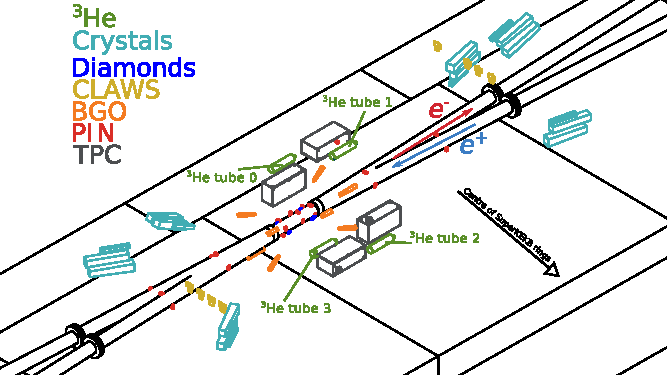
\includegraphics[width=\textwidth]{images/BEAST-Phase1-LineArt-16-9_IsoMetric-Colours-EmbeddedText}
	\caption[CAD rendering of BEAST~II in Phase~I]{CAD rendering of BEAST~II showing colour-coded locations of all subdetectors. The support structure is omitted for clarity~\cite{BEASTPAPER}.}
	\label{fig:beastRender}
\end{figure}

%\begin{figure}[ht!]
%\centering
%%% Creator: Inkscape 0.91_64bit, www.inkscape.org
%% PDF/EPS/PS + LaTeX output extension by Johan Engelen, 2010
%% Accompanies image file 'BEAST-Phase1-MasterCoordinateSystem-v2.pdf' (pdf, eps, ps)
%%
%% To include the image in your LaTeX document, write
%%   \input{<filename>.pdf_tex}
%%  instead of
%%   \includegraphics{<filename>.pdf}
%% To scale the image, write
%%   \def\svgwidth{<desired width>}
%%   \input{<filename>.pdf_tex}
%%  instead of
%%   \includegraphics[width=<desired width>]{<filename>.pdf}
%%
%% Images with a different path to the parent latex file can
%% be accessed with the `import' package (which may need to be
%% installed) using
%%   \usepackage{import}
%% in the preamble, and then including the image with
%%   \import{<path to file>}{<filename>.pdf_tex}
%% Alternatively, one can specify
%%   \graphicspath{{<path to file>/}}
%% 
%% For more information, please see info/svg-inkscape on CTAN:
%%   http://tug.ctan.org/tex-archive/info/svg-inkscape
%%
\begingroup%
  \makeatletter%
  \providecommand\color[2][]{%
    \errmessage{(Inkscape) Color is used for the text in Inkscape, but the package 'color.sty' is not loaded}%
    \renewcommand\color[2][]{}%
  }%
  \providecommand\transparent[1]{%
    \errmessage{(Inkscape) Transparency is used (non-zero) for the text in Inkscape, but the package 'transparent.sty' is not loaded}%
    \renewcommand\transparent[1]{}%
  }%
  \providecommand\rotatebox[2]{#2}%
  \ifx\svgwidth\undefined%
%    \setlength{\unitlength}{229.9bp}%
    \setlength{\unitlength}{\textwidth}	
    \ifx\svgscale\undefined%
      \relax%
    \else%
      \setlength{\unitlength}{\unitlength * \real{\svgscale}}%
    \fi%
  \else%
    \setlength{\unitlength}{\svgwidth}%
  \fi%
  \global\let\svgwidth\undefined%
  \global\let\svgscale\undefined%
  \makeatother%
  \begin{picture}(1,1)%
    \put(0,0){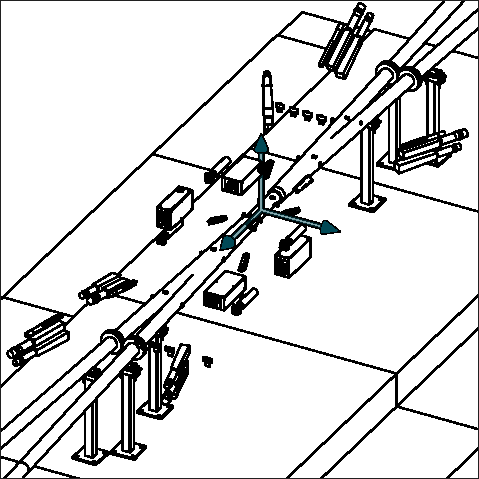
\includegraphics[width=\unitlength,page=1]{images/BEAST-Phase1-MasterCoordinateSystem-v2.pdf}}%
    \put(0.43004132,0.49912999){\color[rgb]{0       , 0.282353, 0.333333} $z$}%
    \put(0.67935308,0.47502588){\color[rgb]{0       , 0.282353, 0.333333} $x$}%
    \put(0.56545083,0.68934171){\color[rgb]{0       , 0.282353, 0.333333} $y$}%
    \put(0,0){
\includegraphics[width=\unitlength,page=1]{images/BEAST-Phase1-MasterCoordinateSystem-Arrows.pdf}}%
    \put(0.3617227,0.3072984){\color[RGB]{232,44,42}$e^{-}$}%
    \put(0.31324316,0.40748951){\color[RGB]{4,144,188}$e^{+}$}%
  \end{picture}%
\endgroup%

%\caption[CAD render of BEAST~II in Phase~I]{CAD render of BEAST~II showing locations of all subdetectors. Support structure is omitted for clarity}
%\label{fig:beastRender} ~\cite{BEASTPAPER}
%\end{figure}


\begin{table}[ht]
	\centering
	\begin{tabular}{ llc }
		Subdetector	&	Purpose				&	Number of devices	\\	\hline \hline
		PINs		&	Ionizing radiation		&	64	\\	
		Crystals	&	Injection and 
					Machine backgrounds		&	18	\\	
		\He tubes	&	Thermal neutron detection	&	4	\\	
		Time projection
		 chambers	&	Fast neutron detection		&	2	\\	
		CLAWS		&	Fast injection background	&	8	\\	
		Diamonds	&	Radiation dose monitor		&	4	\\	
		BGO		&	Machine backgrounds		&	8	\\	\hline
	\end{tabular}
	\caption[Summary of BEAST~II Phase~I detectors]{Summary of BEAST~II Phase~I detectors.}
	\label{tab:beastPhase1}
\end{table}


\section{Crystals}
\label{sec:CSI}

	The crystal subsystem consists of six crystal boxes, three on each side of the interaction region (IR). Each box contains three crystals: pure caesium iodide (CsI), thallium doped CsI (CsI(Tl)), and cerium-doped lutetium yttrium orthosilicate (LYSO). When charged particles enter these crystals, they generate showers and produce visible light with an intensity proportional to the energy deposited by the particle. Photomultiplier tubes attached to the end of the crystals collect this light and produce a signal.


\section{BGO}

	Eight bismuth germanate (\textbf{B}i$_4$\textbf{G}e$_3$\textbf{O}$_{12}$ - BGO) crystals (four in the forward region, four in the backward region) are installed with their long axes pointing at the interaction point (IP). In Phase~II of BEAST~II, these will measure the radiative Bhabha events. In Phase~I, they act as a general monitor of radiation. The BGO crystals measure radiation in the same way as the crystals discussed in \S~\ref{sec:CSI}. 

\section{TPCs}
\label{sec:TPCs}
	
	The fast neutron \textbf{T}ime \textbf{P}rojection \textbf{C}hambers (TPCs) detect fast neutrons by measuring tracks from recoiling alpha particles. The detectors themselves are rectangular boxes filled with helium. When the alpha particles recoil, they produce ionization tracks which drift to a sensor at the end of the box. There were four TPCs in place in Phase~I of BEAST~II, two of which were operating. 



\section{Diamonds}

	Four $(4.5\times4.5\times0.5$mm$)^2$ diamond sensors are mounted to the beampipe near the IR. The purpose of these sensors is to provide an instantaneous and integrated measurement of the dose near the IR. The diamond crystals have electrodes deposited on opposite sides. A potential difference applied between the electrodes produces an electric field of approximately 1 V/$\mu $. When charged particles cross the diamond, an electron-hole pair is produced for each 13 eV of energy that is deposited. These electron-hole pairs produce a current in the diamond, which is measured to determine the dose.


\section{PINs}

	An array of PIN (three layers of semiconductor: \textbf{P}-doped, \textbf{I}ntrinsic, and \textbf{N}-doped) diodes at various locations around BEAST~II provide a simple and inexpensive measurement of ionizing radiation. The radiation produces an increase in the dark current of the diodes, which is measured to provide the dose. Half of the PIN diodes are coated in a thin layer of gold paint, which reduces the X-ray dose. A comparison between shielded and unshielded diodes gives a direct measurement of the syncrotron radiation dose. Each PIN subdetector contains two diodes (one gold coated, and one not) and a temperature monitor encased in an aluminum block. Eight sets of four blocks are placed at various locations surrounding the beampipe, for a total of 64 channels.

\section{CLAWS}

	The s\textbf{C}intillation \textbf{L}ight \textbf{A}nd \textbf{W}aveform \textbf{S}ensors (CLAWS) detector system measures backgrounds, in particular those caused by injection. It consists of eight scintillator tiles read out by silicon photomultipliers. The system has a 0.8 ns sampling rate, making it ideal for measuring the fast injection signals. These results are sent to the SuperKEKB control room, providing fast feedback of accelerator performance.


\section{\He Tubes}

	The \he tubes provide thermal neutron detection, and are discussed in detail in Chapter \ref{chap:he3tube}.


\section{Phase~II}

	In the fall of 2017, Phase~II of BEAST~II will begin. During this phase, the Belle~II detector (without the VXD systems) will be rolled into the IR. Phase~I devices will continue to be used in this phase, with the exception of the crystal boxes, as the ECL will take similar measurements. In addition, there will be two new subdetectors: \textbf{F}E-I4 \textbf{A}TLAS \textbf{N}ear \textbf{G}amma \textbf{S}ensors (FANGS) and \textbf{P}ixelated \textbf{L}adder with \textbf{U}ltra-low \textbf{M}aterial \textbf{E}mbedding (PLUME). The CLAWS, FANGS, PLUME, and BGO systems will be installed in the VXD space. The TPCs and \he tubes will go into the dock spaces as shown in Fig \ref{fig:dockSpace}. During this phase, the 1.5 T magnetic field of Belle~II will be turned on.

\begin{figure}[htb]
	\centerfloat
		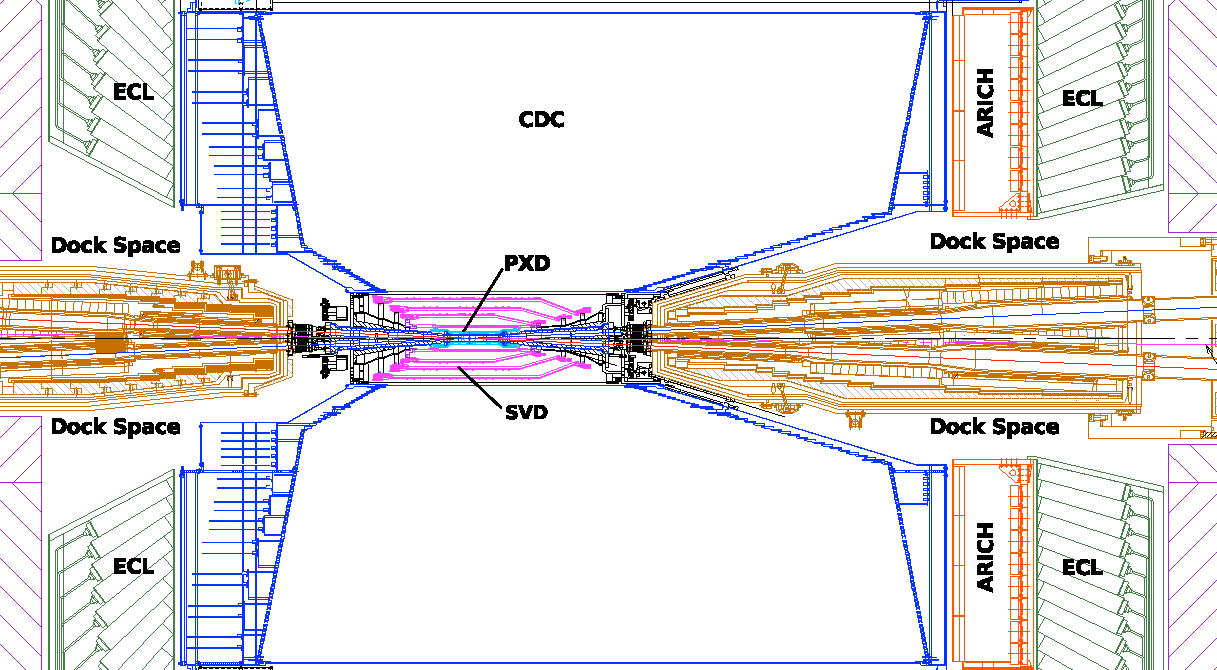
\includegraphics[width=\textwidth]{images/Belle-ll-DockSpace_text}
	\caption[Belle~II dock spaces]{Belle~II dock spaces.}		
	\label{fig:dockSpace}
\end{figure}



















